\chapter{量子光通信的理论基础}

\section{电磁场的量子态描述}
\subsection{相干态}
通信中常用相干光来传递信息,它可以用一个正弦波来表示。
不失一般性,可以用线偏振的电场来实现\cite{djordjevic2010fundamentals},
\begin{equation}
\bm{E}(t) = \bm{p} A e^{j\omega t + \phi}.
\end{equation}
上式中,符号$\bm{p}$、$A$、$\omega$和$\phi$分别对应偏振矢量、幅度、频率和相位。
要传递的信息被调制在场的这四个要素上面。
在本文中,主要关注的是对幅度和相位的调制。
这两个要素可以用一个复振幅来描述
\begin{equation}
\alpha = A e^{j\phi}.
\end{equation}
也可以用相空间复平面中的一个点来表示该复振幅,这种图像称作星座图。
图\ref{fig:signals}展示了OOK、BPSK、QPSK、16-QAM四种常见的调制信号的星座图。

\begin{figure}
\centering
  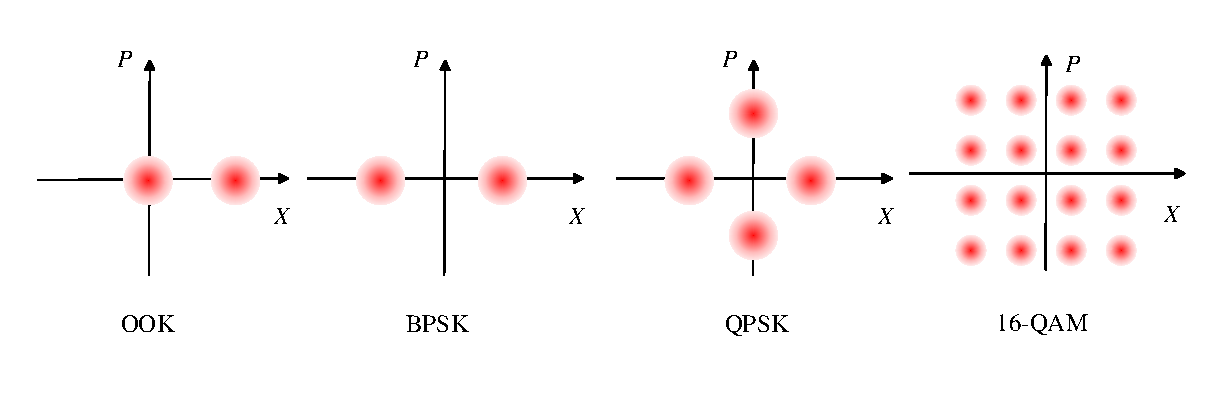
\includegraphics[width=\textwidth]{figures/chap2/signals}
  \caption{常见的四种调制信号星座图}
  \label{fig:signals}
\end{figure}

在量子力学中,电磁场被量子化为若干个不同模式、不同频率的光子\cite{gerry2005introductory,helstrom1976quantum,mandel1995optical}。
单模电磁场的哈密顿量可以表示为
\begin{equation}
\hat{H} = \hbar \omega (\hat{a}^\dagger \hat{a} + \frac{1}{2}).
\end{equation}
其中$\hat{a}^\dagger$和 $\hat{a}$ 分别是产生湮灭算符,
乘积$\hat{a}^\dagger \hat{a}$是粒子数算符,他的本振态是Fork态$\ket{n}$。
\begin{equation}
\hat{a}^\dagger \hat{a} \ket{n} = n \ket{n}.
\end{equation}

通信中常用的单模相干光脉冲可以用单模相干态$\ket{\alpha}$来描述,它是湮灭算符的本振态
\begin{equation}
\hat{a} \ket{\alpha} = \alpha \ket{\alpha}.
\end{equation}
在Fork态表象中,相干态可以表达为
\begin{equation}
\ket{\alpha} = \exp(-\frac{1}{2}|\alpha|^2) \sum_{n=0}^\infty \frac{\alpha^n}{\sqrt{n!}} \ket{n}.
\end{equation}
如果用光子计数器进行探测,相干态$\ket{\alpha}$探测到的光子数不是一个固定的值,
而是服从泊松分布
\begin{equation}
P_n = |\bra{n}\ket{\alpha}|^2 = \exp(-|\alpha|^2) \frac{|\alpha|^{2n}}{n!} .
\end{equation}
它的平均光子数由
\begin{equation}
\bar{n} = |\alpha|^2
\end{equation}
给出。相干态参数${\alpha}$可以是任何复数,具有复振幅的意义\cite{glauber1963coherent}。

数学上也常常用密度矩阵来表示信号\cite{wt2001qm},相干态$\ket{\alpha}$也可以用密度矩阵表示为
$\ket{\alpha}\bra{\alpha}$。



\subsection{位移操作}

\begin{figure}
\centering
  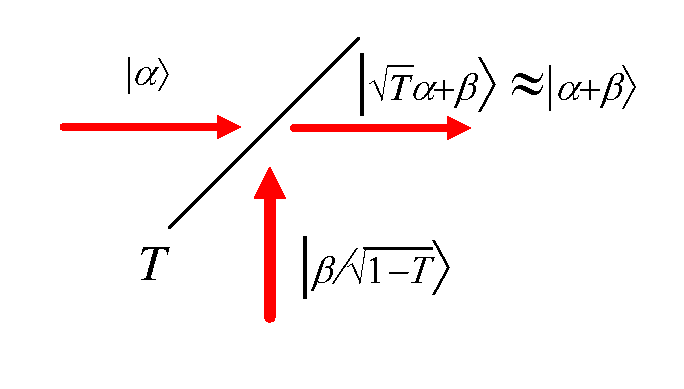
\includegraphics[height=5cm]{figures/chap2/displacement-operator}
  \caption{用波束分束器实现位移操作示意图}
  \label{fig:diaplacement}
\end{figure}

相干态可以通过位移操作进行变换,位移算符定义为\cite{glauber1963coherent,gerry2005introductory,helstrom1976quantum,mandel1995optical}
\begin{equation}
\hat{D}(\alpha) = \exp(\alpha \hat{a}^\dagger - \alpha^* \hat{a}).
\end{equation}
利用位移算符,相干态可以通过对真空态$\ket{0}$位移得到
\begin{equation}
\hat{\alpha} = \hat{D}(\alpha) \ket{0}.
\end{equation}
两个相干态之间也可以通过位移操作进行转换
\begin{equation}
\hat{D}(\beta) \ket{\alpha} = \ket{\alpha + \beta} .
\end{equation}


在实验当中,常用一个相位稳定干涉仪或者波束分束器来实现\cite{cook2007optical,becerra2013experimental,lau2006binary,paris1996displacement}。
图\ref{fig:diaplacement}显示的是利用一个高透过率的波束分束器,
将两个入射场混合输出,近似实现了对其中一个入射场的位移操作。
这种方案在量子接收机实验中经常见到。

\section{经典光通信的接收方案}

\subsection{引言}
在经典光通信中,有三类常见的接收方案,他们分别是
直接检测、零差接收和外差接收。
这三种接收方案受散粒噪声的制约,
使得每一种接收方案存在一个经典极限
——标准量子极限(Standard Quantum Limit)。
接下来,我们简单介绍一下每一种接收方案的具体实现方案。

\subsection{直接检测}

在所有的调制方案中,有一类采用脉冲的有无对信息进行编码,
比如开关键控(OOK)和脉冲位置调制(PPM)。
OOK调制将符号0编码为没有光脉冲,
而将符号1编码为有脉冲;PPM调制则将信息编码到脉冲所在的位置上。
对于这样一类的调制方案,经典光通信中常采用直接检测方案进行探测。
如图\ref{fig:DD}所示,直接检测方案直接探测信号光的强度,
来判断是否存在光脉冲或者光脉冲的幅度\cite{gagliardi1976optical,gagliardi1998optical}。
这种方案可以利用一个光电探测器或单光子探测器实现。
探测器可以输出探测到的光子数目,理想情况下,
对于给定的相干态,探测到$n$个光子的概率
\begin{equation}
\Pr(N = n| \ket{\alpha}) = \frac{|\alpha|^{2n}}{n!} e^{-|\alpha|^2}
\label{eq:dd-prob}
\end{equation}
一般地,对于信号矢态为$\ket{\phi}$的情况下,检测概率为
\begin{equation}
\Pr(N = n| \ket{\phi}) = |\bra{n}\ket{\phi}|^2
\end{equation}



\begin{figure}
\centering
  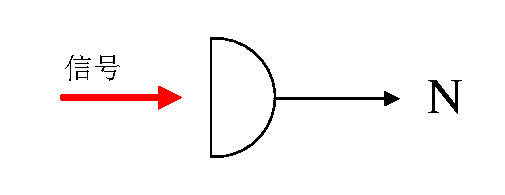
\includegraphics[scale=1]{figures/chap2/DD.pdf}
  \caption{直接检测示意图}
  \label{fig:DD}
\end{figure}


\subsection{零差接收}
零差接收机是一种相干检测方案,如图\ref{fig:HD}所示,
是一种平衡零差接收方案\cite{gagliardi1976optical,gagliardi1998optical}。
这种接收方案和直接检测不同的是,
需要一个本振。对于零差接收本振频率和信号频率一致。
通常本振强度$a_{LO}$远大于信号强度$a_S$,
两路信号通过一个50:50的分束器,
在两个输出口得到两路新的信号$a_+$和$a_-$,满足关系式
\begin{equation}
a_\pm = \frac{a_S \pm a_{LO}}{\sqrt{2}}.
\end{equation}
这两路信号被光电探测器接收,得到两路光电流$i_\pm$。
这两路电流通过一个放大系数为$\frac{1}{K}=\frac{1}{2q\sqrt{N_{LO}}}$的差分放大器,
最后通过一个低通滤波器积分得到输出统计量
\begin{equation}
\alpha_\theta = \frac{N_+ - N_-}{2\sqrt{N_{LO}}}.
\end{equation}
这里假定所有的器件都是理想的。当$N_{LO} \rightarrow \infty$时,
输出统计量服从高斯分布
\begin{equation}
\alpha_\theta \sim N(Re(ae^{-j\theta}), \frac{1}{4}).
\end{equation}
其中$\theta$是本振与信号的相位差。
这种测量方案,用量子力学算符可以用湮灭算符描述为\cite{yuen1980optical,mandel1995optical}
\begin{equation}
\hat{\alpha}_\theta = \Re(\hat{a}_S e^{-j\theta}).
\end{equation}


\begin{figure}
\centering
  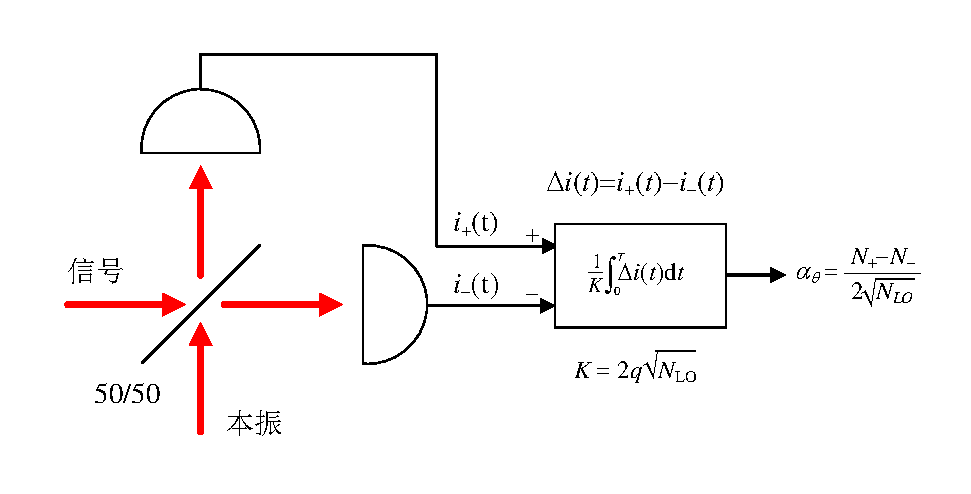
\includegraphics[width=0.8\textwidth]{figures/chap2/homodyne-receiver.pdf}
  \caption{平衡零差检测示意图}
  \label{fig:HD}
\end{figure}

\subsection{外差接收}
在上一小节,我们已经介绍了零差接收方案。
另外一种相干接收方案是外差接收\cite{gagliardi1976optical,gagliardi1998optical},
它采用了与信号频率不同的本振。
图\ref{fig:HeD}是一种平衡外差接收机示意图,
在这种外差接收机中,频率为$\omega$的信号场$a_S$
与频率为$\omega - \omega_{IF}$的强本振场$a_{LO}$
通过一个50:50的分束器混合。
混合后经过光电探测器,得到两路以中频$\omega_{IF}$震荡的电流$i_\pm$。
这两路电流经过一个放大系数为$\frac{1}{K'}=\frac{1}{q\sqrt{N_{LO}}}$的差分放大器,
最后解调出两个正交幅度$\alpha_1$和$\alpha_2$。
假定所有的器件都是理想的,当$N_{LO} \rightarrow \infty$时,
这两个统计量统计独立,分别服从高斯分布
\begin{equation}
\alpha_i \sim N(a_{S_i}, \frac{1}{2}).
\end{equation}
其中$a_{S_1}=\Re(a_S)$和$a_{S_2}=\Im(a_S)$分别是信号场的两个正交幅度。
这种测量方案,用量子力学算符湮灭算符可以描述为\cite{yuen1980optical,mandel1995optical}
\begin{equation}
\hat{\alpha}_1 + j \hat{\alpha}_2 = \hat{a}_S.
\end{equation}



\begin{figure}
\centering
  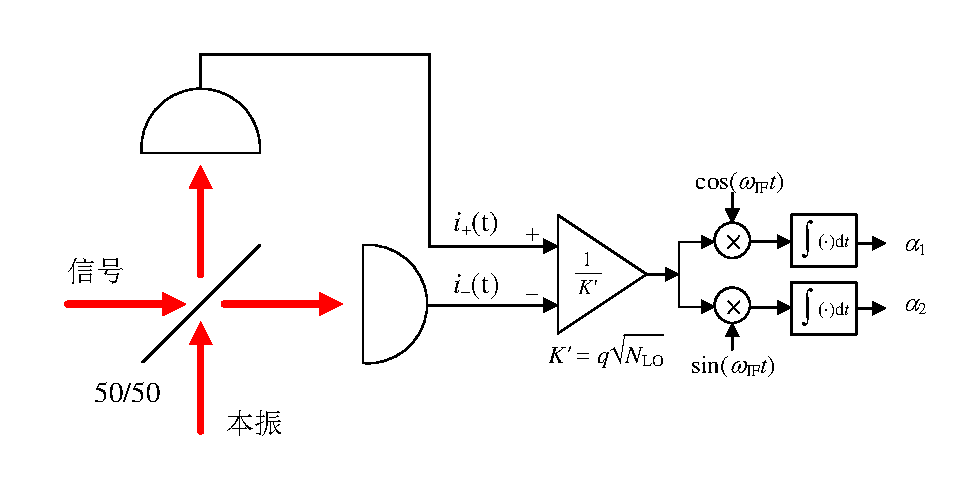
\includegraphics[width=0.8\textwidth]{figures/chap2/heretrodyne-receiver.pdf}
  \caption{平衡外差检测示意图}
  \label{fig:HeD}
\end{figure}


\section{量子检测与估计理论}
\subsection{经典最优检测}
通信系统通常由发送端、信道和接收端三个部分组成。
对某种特定的通信方案,发送端通常从$M$个符号中选择一个发送出去。
我们称一个假设$H_j (j=1,2,...,M)$是指发送的是第$j$个符号。
对于这$M$个符号,我们赋予它们一个先验概率$\zeta_j$,
先验概率满足归一化条件
\begin{equation}
\sum_{j=1}^M \zeta_j = 1.
\end{equation}


在通信的接收端,接收机对电磁场进行探测,可以得到一些统计量。
例如在前面介绍的三种经典监测方案,输出的统计量分别是光子数目、
$\alpha_\theta$、$\{\alpha_1, \alpha_2\}$。
由于量子涨落或者噪声的影响,对于给定的发送信号,
这些统计量通常不是一个固定的值,而是一个随机变量。
一般的,我们假设输出统计量是一个随即向量$\bm{v} = (v_1, v_2, ..., v_n)$。
当发送第$j$个符号时,
假定它的联合分布为$p_j(\bm{v}) = p_j(v_1, v_2, ..., v_n)$。



\subsection{量子最优检测}






\subsection{平方根检测}







\section{现有的量子接收机简介}

\subsection{二进制信号量子接收机}




\subsection{PSK信号量子接收机}





\subsection{其它类型量子接收机}






\section{量子信道编码理论}

\subsection{Holevo容量}






\subsection{常见的量子编码方案}





